\section{الگوریتم های برنامه ریزی مسیر}
مسئله پیدا کردن کوتاهترین مسیر از یک راس به راس دیگر در یک گراف متصل در کاربرد های
 مختلف به خصوص در اینترنت برای جستجوی  مسیر بهینه برای پاکت های داده مورد علاقه است.
کلمه ی
\textbf{کوتاهترین}
در اینجا به معنی کمترین هزینه جمعی یال ها است که می تواند فاصله فیزیکی، تاخیر و هر اندازه دیگری که برای یک کاربرد خاص مد نظر است باشد. یک مثال از گراف با یال های دلخواه در شکل
\ref{fig:graph}
نشان داده شده است. 

\begin{figure}[H]
  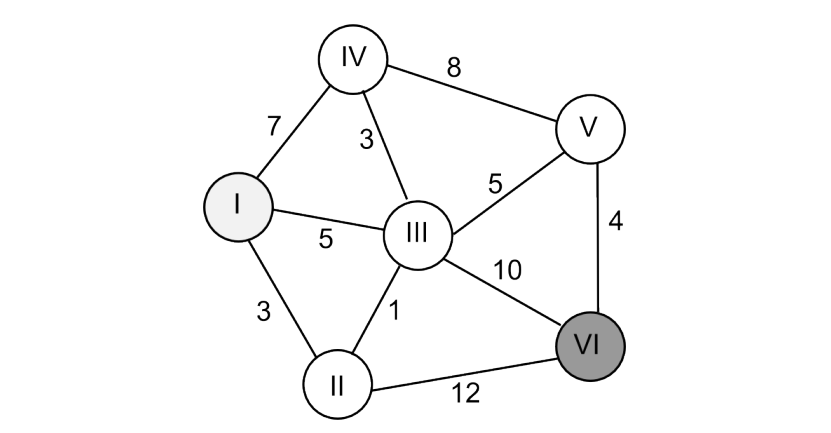
\includegraphics[width = \textwidth]{images/graph.png}
  \caption{مسئله برنامه ریزی مسیر از راس
  \rom{1}
  به راس
  \rom{2}
  .
  \\
  کوتاهترین میسر 
  $\rom{1}-\rom{2}-\rom{3}-\rom{5}-\rom{6}$
  به طول ۱۳ است
  }
  \label{fig:graph}
\end{figure}
\subsection{تجسم ربات}
برای کار کردن با تجسم فیزیکی جسم که می تواند پروسه برنامه ریزی مسیر را  پیچیده کند، ربات به جرم
 نقطه ایی کاهش یافته و موانع به اندازه بزرگترین فاصله نقطه ایی روی جسم  که از مرکز جسم فاصله
 دارد به آن مقدار  در جهت های مختلف اضافه می شود. این نمایش به 
\lr{\textbf{configuration space}}
معروف است. یک مثال در شکل
\ref{fig:conf-space}
نشان داده شده است.
\lr{configuration space}
می تواند به عنوان پایه برای نقشه شبکه ایی یا پیوسته به کار رود.
\begin{figure}[H]
  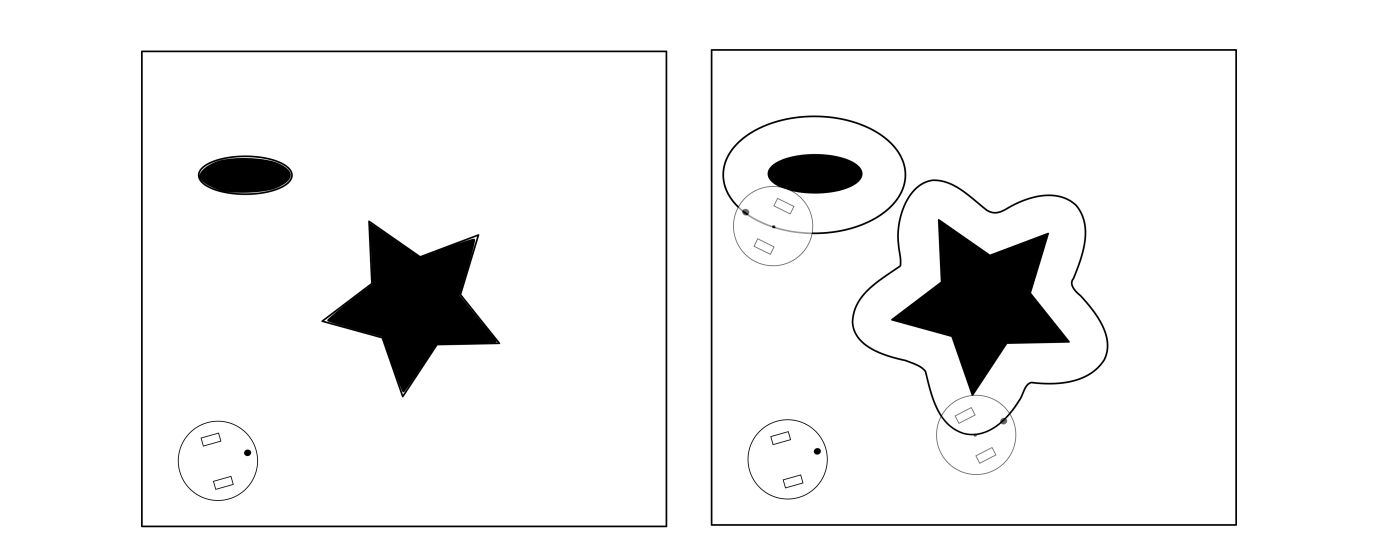
\includegraphics[width = \textwidth]{images/conf-space.png}
  \caption{
  یک نقشه با موانع با نمایش 
  \lr{configuration space}
  آن که با اضافه کردن فضای تصرف ربات به موانع بدست می آید.
  }
  \label{fig:conf-space}
\end{figure}
\subsection{الگوریتم دایجسترا}
یکی از اولین و ساده ترین الگوریتم ها، الگوریتم دایجسترا است. الگوریتم به این شکل است که از راس
 ابتدایی شروع می کنیم، همه همسایه های مستقیم با هزینه رفتن به هر کدام مشخص می شود. سپس
با راس با کوچکترین هزینه شروع کرده و تمام همسایه های آن با هزینه آن ها از راس شروع  مشخص
 می شود و این عمل تا زمانی که راسی که انتخاب می شود راس پایان باشد ادامه میدهیم و پس از آن ربات
 میتواند یال هایی که از آن به پایان رسیدم رو دنبال کند.
در شکل 
\ref{fig:graph}
الگوریتم ابتدا راس های 
\rom{2}
،
\rom{3}
و
\rom{4}
با هزینه های به ترتیب ۳، ۵ و ۷ مشخص می شوند. سپس شروع به جستجوی تمام یال های راس 
\rom{2}
می کند که تا اینجا کمترین هزینه را داشته است. این کار باعث پیدا شدن این می شود که راس
\rom{3}
با هزینه کمتری 
$3+1<5$
قابل دسترسی است و این راس با هزینه ی ۴ قابل  دسترسی است. دایجسترا به منظور اینکه ارزیابی کامل راس
\rom{2}
نیاز دارد که یال های باقی مانده را قبل از رفتن به راس بعدی بررسی کند. بنابراین راس 
\rom{6}
با 
$3+12=15$
مشخص می شود.

حال راس با کمترین هزینه راس 
\rom{3}
است. حال می توانیم راس 
\rom{6} 
را با ۱۴ که کوچکتر از مقدار قبلی آن ۱۵ است مشخص کنیم و راس
\rom{5}
با 
$4+5=9$
برچسب می گذاریم و همینطور راس 
\rom{4}
با 
$4+3=7$
باقی می ماند. هرچند که ما دو مسیر به هدف پیدا کردیم که یکی از آنها بهتر است اما تا زمانی که راس 
هایی با یال های غیر بررسی شده و هزینه های کمتر از ۱۴ وجود دارد، ادامه می دهیم.
در واقع، با ادامه جستجو از راس
\rom{5}
به کوتاهترین مسیر 
$\rom{1}-\rom{2}-\rom{3}-\rom{5}-\rom{6}$
  به طول ۱۳ است با هیچ راس دیگری برای جستجو باقی می مانیم.
به این دلیل که دایجسترا تا زمانی که راس دیگری با هزینه کمتر از هزینه ایی که تا هر نقطه زمان به هدف
 پیدا شده تمام نمی شود، می توانیم مطمئن باشیم کوتاهترین مسیر در صورت وجود، پیدا می شود و
 الگوریتم کامل
\lr{(complete)}
 است.
از آنجایی که دایجسترا ابتدا همیشه راس هایی با کمترین هزینه را بررسی می کند، محیط به صورت موجی است که از راس شروع سرچشمه می گیرد و به هدف می رسد. این روش در شرایط خاصی که هدف از راس ابتدایی دور است به شدت غیر بهینه است. با اضافه کردن چند راس به سمت چپ شکل
\ref{fig:graph}
قابل لمس است.
دایجسترا این راس ها را تا زمانی که  هزینه آنها از کمترین هزینه که به هدف پیدا شده است، بالاتر برود جستجو می کند. این زمانی که الگوریتم روی شبکه ها اجرا می شوند قابل مشاهده است همانطور که در شکل 
\ref{fig:dijkstra}
نشان داده شده است.

\begin{figure}[H]
  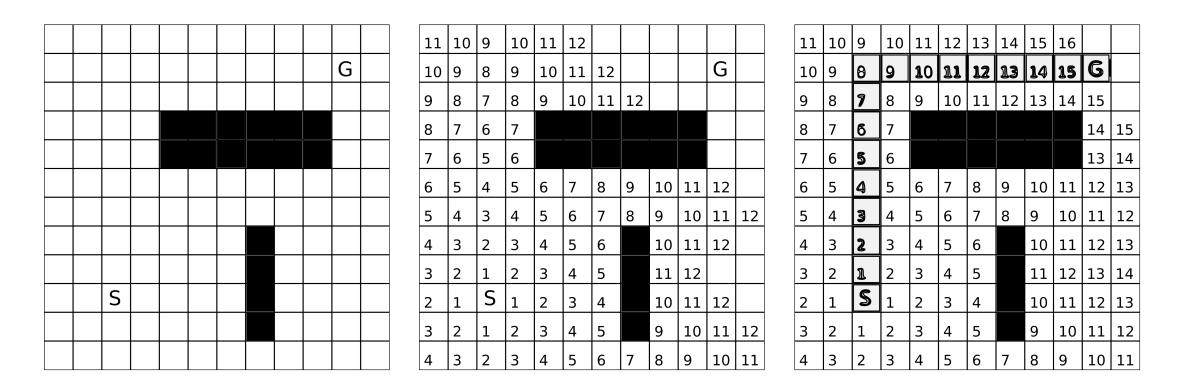
\includegraphics[width = \textwidth]{images/dijkstra.png}
  \caption{
 پیدا کردن کوتاهترین مسیر از  
  \lr{\textbf{S}}
  به
  \lr{\textbf{G}}
با این شرط که ربات فقط می تواند بالا-پایین و چپ-راست برود و هزینه یک برای برای هر حرکت.
  }
  \label{fig:dijkstra}
\end{figure}
\subsection{الگوریتم A*}
به جای جستجو در تمام جهت ها، دانش تقریبی از موقعیت هدف در پرهیز از جستجوی راس ها که کاملا از
 نظر عامل انسانی غیر منطقی است میتواند کمک کند. چنین دانشی که همچنین مشاهده گری دارد از طریق تابع 
\lr{heuristic}
کدگذاری می توان شد.
برای مثال ما می توانیم به راس هایی که فاصله تقریبی کمتری از هدف دارند اولویت بیشتری بدهیم. در این روش نه تنها فاصله واقعی تا راس ها بلکه  فاصله تقریبی تا هدف هم در نظر میگیریم. برای مثال این تقریب می تواند فاصله اقلیدسی یا منهتنی بین راس مورد نظر و هدف باشد. این الگوریتم با نام 
\lr{A*}
معروف است. با توجه به شرایط، این الگوریتم از الگوریتم دایجسترا می تواند خیلی سریع تر عمل کند، و در بدترین شرایط بازده آن یکسان باشد. این در شکل
\ref{fig:astar}
نشان داده شده.  فاصله منهتنی به عنوان تابع 
\lr{heuristic} 
استفاده شده است.
\begin{figure}[H]
  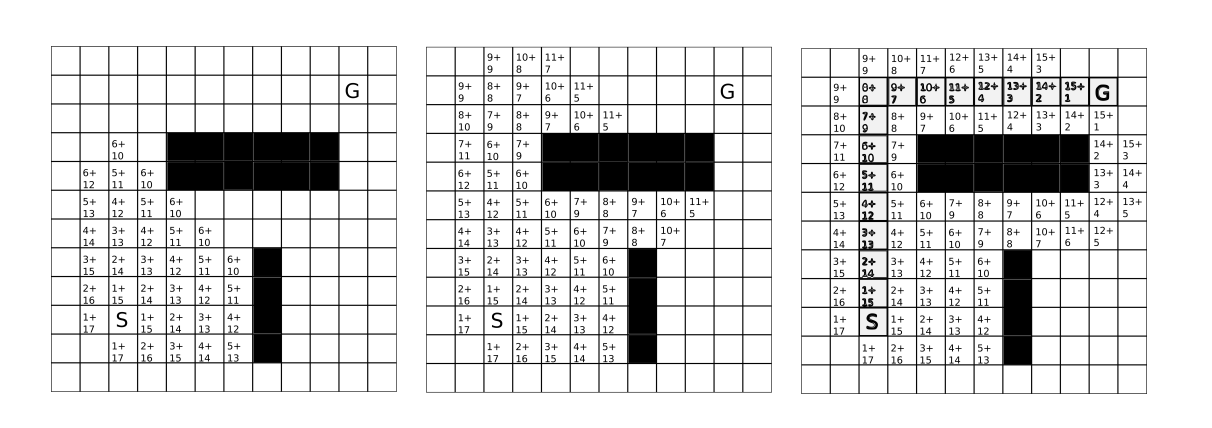
\includegraphics[width = \textwidth]{images/astar.png}
  \caption{
 پیدا کردن کوتاهترین مسیر از  
  \lr{\textbf{S}}
  به
  \lr{\textbf{G}}
با این شرط که ربات فقط می تواند بالا-پایین و چپ-راست برود و هزینه یک برای برای هر حرکت.
  }
  \label{fig:astar}
\end{figure}
\par
\lr{A*}
در صورت اینکه فضای جستجو بزرگ باشد، وضوح تصویر برای انجام عمل نیاز باشد و یا ابعاد مسئله جستجو بالا باشد،  هزینه محاسباتی بالایی خواهد داشت. جواب این مسائل در الگوریتم برنامه ریزی مسیر بر پایه نمونه برداری
\lr{(Sampling-based)}
برآورده شده است. که در بخش بعدی بررسی خواهیم کرد. 
\subsection{پیاده سازی الگوریتم 
\lr{A*}
در پایتون
}
پیاده سازی الگوریتم
\lr{A*}
چندان پیچیده نیست. مسئله ایی که اهمیت دارد این است که در این الگوریتم ما یک صف اولویت خواهیم داشت که بر اساس تابع 
$f(n) = g(n) + h(n)$
(که در آن 
$g(n)$
کمترین هزینه پیدا شده از شروع تا گره 
$n$
و 
$h(n)$
 تابع
 \lr{heuristic}
 است) در هر مرحله گره ها را انتخاب و بررسی می کنیم. تا گره ایی که از صف خارج می شود گره ی هدف باشد. در این مثال فاصله منهتنی بین راس مورد نظر تا گره هدف به عنوان تابع
 \lr{heuristic}
 انتخاب شده است. در کد زیر ورودی تابع شامل نقشه که ماتریسی از صفر و یک ها است که موانع را در صورت وجود با یک نشان می دهد و نقطه شروع و هدف است. و خروجی تابع مسیر بهینه، شامل دنباله ایی از موقعیت ها از گره شروع تا پایان خواهد بود.
\begin{latin}
\pythonexternal[caption={\textbf{A*}},
    label={list:astar}]{codes/astar.py}
\end{latin}
این تیکه کد را با یک تغییر ساده می توان به الگوریتم دایجسترا تبدیل کرد. فقط کافی است 
$f(n)=g(n) $
بگذاریم و در قطعه کد بالا  با تغییر کد خط ۸ به 
\\
\lr{    f = lambda n: n[2]}
\\
به این نتیجه خواهیم رسید.
\begin{figure}[H]
    \centering
    
\begin{tabular}{cc}
   \subfloat[]{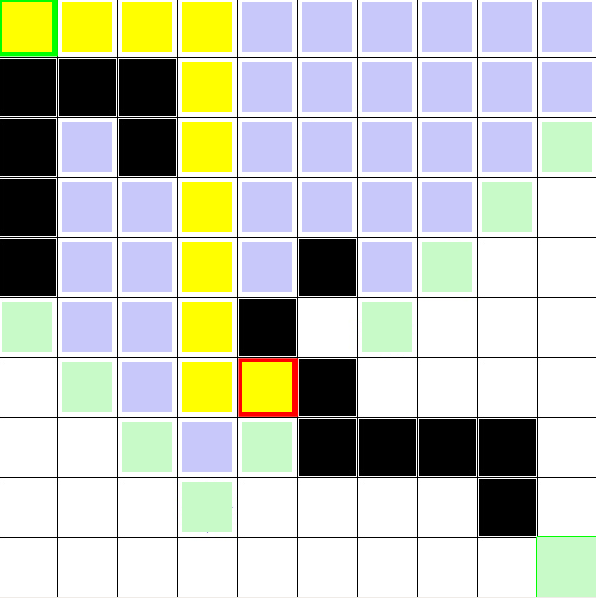
\includegraphics[width = 0.5\textwidth]{images/python-dijkstra.png}} &
\subfloat[]{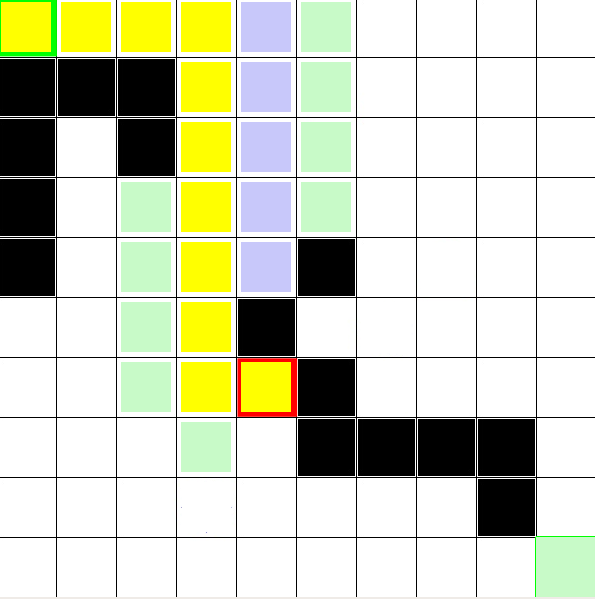
\includegraphics[width = 0.5\textwidth]{images/python-astar.png}} 
\end{tabular}
    \caption{
    خانه شروع 
    $(0,0)$
    خانه هدف
      $(7,5)$
      مسیر زرد رنگ مسیر بهینه را نشان می دهد،
      خانه های آبی خانه های مورد بررسی شده ی الگوریتم را نشان می دهد،
      خانه های سبز گره هایی که داخل صف که بررسی نشده اند را نشان میدهد،
    (آ)اجرای الگوریتم دایجسترا روی 
    \lr{gird map}
    (ب)اجرای الگوریتم
    \lr{A*}
    روی 
    \lr{gird map}
    }
    \label{fig:execute}
\end{figure}

